\documentclass[twoside]{book}

% Packages required by doxygen
\usepackage{fixltx2e}
\usepackage{calc}
\usepackage{doxygen}
\usepackage[export]{adjustbox} % also loads graphicx
\usepackage{graphicx}
\usepackage[utf8]{inputenc}
\usepackage{makeidx}
\usepackage{multicol}
\usepackage{multirow}
\PassOptionsToPackage{warn}{textcomp}
\usepackage{textcomp}
\usepackage[nointegrals]{wasysym}
\usepackage[table]{xcolor}

% Font selection
\usepackage[T1]{fontenc}
\usepackage[scaled=.90]{helvet}
\usepackage{courier}
\usepackage{amssymb}
\usepackage{sectsty}
\renewcommand{\familydefault}{\sfdefault}
\allsectionsfont{%
  \fontseries{bc}\selectfont%
  \color{darkgray}%
}
\renewcommand{\DoxyLabelFont}{%
  \fontseries{bc}\selectfont%
  \color{darkgray}%
}
\newcommand{\+}{\discretionary{\mbox{\scriptsize$\hookleftarrow$}}{}{}}

% Page & text layout
\usepackage{geometry}
\geometry{%
  a4paper,%
  top=2.5cm,%
  bottom=2.5cm,%
  left=2.5cm,%
  right=2.5cm%
}
\tolerance=750
\hfuzz=15pt
\hbadness=750
\setlength{\emergencystretch}{15pt}
\setlength{\parindent}{0cm}
\setlength{\parskip}{3ex plus 2ex minus 2ex}
\makeatletter
\renewcommand{\paragraph}{%
  \@startsection{paragraph}{4}{0ex}{-1.0ex}{1.0ex}{%
    \normalfont\normalsize\bfseries\SS@parafont%
  }%
}
\renewcommand{\subparagraph}{%
  \@startsection{subparagraph}{5}{0ex}{-1.0ex}{1.0ex}{%
    \normalfont\normalsize\bfseries\SS@subparafont%
  }%
}
\makeatother

% Headers & footers
\usepackage{fancyhdr}
\pagestyle{fancyplain}
\fancyhead[LE]{\fancyplain{}{\bfseries\thepage}}
\fancyhead[CE]{\fancyplain{}{}}
\fancyhead[RE]{\fancyplain{}{\bfseries\leftmark}}
\fancyhead[LO]{\fancyplain{}{\bfseries\rightmark}}
\fancyhead[CO]{\fancyplain{}{}}
\fancyhead[RO]{\fancyplain{}{\bfseries\thepage}}
\fancyfoot[LE]{\fancyplain{}{}}
\fancyfoot[CE]{\fancyplain{}{}}
\fancyfoot[RE]{\fancyplain{}{\bfseries\scriptsize Generated by Doxygen }}
\fancyfoot[LO]{\fancyplain{}{\bfseries\scriptsize Generated by Doxygen }}
\fancyfoot[CO]{\fancyplain{}{}}
\fancyfoot[RO]{\fancyplain{}{}}
\renewcommand{\footrulewidth}{0.4pt}
\renewcommand{\chaptermark}[1]{%
  \markboth{#1}{}%
}
\renewcommand{\sectionmark}[1]{%
  \markright{\thesection\ #1}%
}

% Indices & bibliography
\usepackage{natbib}
\usepackage[titles]{tocloft}
\setcounter{tocdepth}{3}
\setcounter{secnumdepth}{5}
\makeindex

% Hyperlinks (required, but should be loaded last)
\usepackage{ifpdf}
\ifpdf
  \usepackage[pdftex,pagebackref=true]{hyperref}
\else
  \usepackage[ps2pdf,pagebackref=true]{hyperref}
\fi
\hypersetup{%
  colorlinks=true,%
  linkcolor=blue,%
  citecolor=blue,%
  unicode%
}

% Custom commands
\newcommand{\clearemptydoublepage}{%
  \newpage{\pagestyle{empty}\cleardoublepage}%
}

\usepackage{caption}
\captionsetup{labelsep=space,justification=centering,font={bf},singlelinecheck=off,skip=4pt,position=top}

%===== C O N T E N T S =====

\begin{document}

% Titlepage & ToC
\hypersetup{pageanchor=false,
             bookmarksnumbered=true,
             pdfencoding=unicode
            }
\pagenumbering{alph}
\begin{titlepage}
\vspace*{7cm}
\begin{center}%
{\Large My Project \\[1ex]\large 1.\+0.\+1 }\\
\vspace*{1cm}
{\large Generated by Doxygen 1.8.13}\\
\end{center}
\end{titlepage}
\clearemptydoublepage
\pagenumbering{roman}
\tableofcontents
\clearemptydoublepage
\pagenumbering{arabic}
\hypersetup{pageanchor=true}

%--- Begin generated contents ---
\chapter{Hierarchical Index}
\section{Class Hierarchy}
This inheritance list is sorted roughly, but not completely, alphabetically\+:\begin{DoxyCompactList}
\item \contentsline{section}{Base}{\pageref{class_base}}{}
\begin{DoxyCompactList}
\item \contentsline{section}{Derived\+One}{\pageref{class_derived_one}}{}
\item \contentsline{section}{Derived\+Two}{\pageref{class_derived_two}}{}
\begin{DoxyCompactList}
\item \contentsline{section}{Derived\+Three}{\pageref{class_derived_three}}{}
\end{DoxyCompactList}
\end{DoxyCompactList}
\item \contentsline{section}{External}{\pageref{class_external}}{}
\begin{DoxyCompactList}
\item \contentsline{section}{Ext\+Implement}{\pageref{class_ext_implement}}{}
\end{DoxyCompactList}
\end{DoxyCompactList}

\chapter{Class Index}
\section{Class List}
Here are the classes, structs, unions and interfaces with brief descriptions\+:\begin{DoxyCompactList}
\item\contentsline{section}{\hyperlink{class_base}{Base} }{\pageref{class_base}}{}
\item\contentsline{section}{\hyperlink{class_derived_one}{Derived\+One} }{\pageref{class_derived_one}}{}
\item\contentsline{section}{\hyperlink{class_derived_three}{Derived\+Three} }{\pageref{class_derived_three}}{}
\item\contentsline{section}{\hyperlink{class_derived_two}{Derived\+Two} }{\pageref{class_derived_two}}{}
\item\contentsline{section}{\hyperlink{class_external}{External} }{\pageref{class_external}}{}
\item\contentsline{section}{\hyperlink{class_ext_implement}{Ext\+Implement} }{\pageref{class_ext_implement}}{}
\end{DoxyCompactList}

\chapter{File Index}
\section{File List}
Here is a list of all files with brief descriptions\+:\begin{DoxyCompactList}
\item\contentsline{section}{Doxy\+Test/\hyperlink{_classes_8cpp}{Classes.\+cpp} }{\pageref{_classes_8cpp}}{}
\item\contentsline{section}{Doxy\+Test/\hyperlink{_classes_8h}{Classes.\+h} }{\pageref{_classes_8h}}{}
\item\contentsline{section}{Doxy\+Test/\hyperlink{_doxy_test_8cpp}{Doxy\+Test.\+cpp} }{\pageref{_doxy_test_8cpp}}{}
\item\contentsline{section}{Doxy\+Test/\hyperlink{stdafx_8cpp}{stdafx.\+cpp} }{\pageref{stdafx_8cpp}}{}
\item\contentsline{section}{Doxy\+Test/\hyperlink{stdafx_8h}{stdafx.\+h} }{\pageref{stdafx_8h}}{}
\item\contentsline{section}{Doxy\+Test/\hyperlink{targetver_8h}{targetver.\+h} }{\pageref{targetver_8h}}{}
\end{DoxyCompactList}

\chapter{Class Documentation}
\hypertarget{class_base}{}\section{Base Class Reference}
\label{class_base}\index{Base@{Base}}


{\ttfamily \#include $<$Classes.\+h$>$}



Inheritance diagram for Base\+:
\nopagebreak
\begin{figure}[H]
\begin{center}
\leavevmode
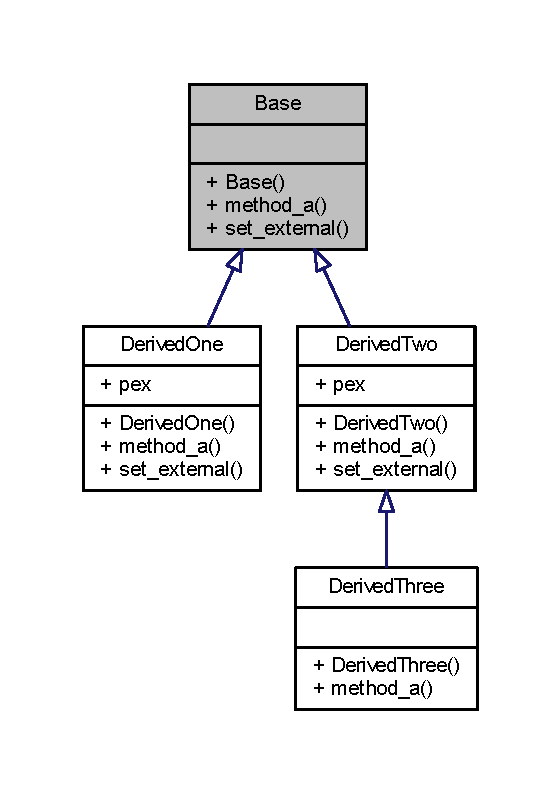
\includegraphics[width=269pt]{class_base__inherit__graph}
\end{center}
\end{figure}


Collaboration diagram for Base\+:
\nopagebreak
\begin{figure}[H]
\begin{center}
\leavevmode
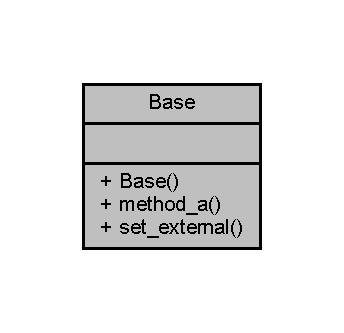
\includegraphics[width=165pt]{class_base__coll__graph}
\end{center}
\end{figure}
\subsection*{Public Member Functions}
\begin{DoxyCompactItemize}
\item 
\hyperlink{class_base_a5ffe0568374d8b9b4c4ec32953fd6453}{Base} ()
\item 
virtual void \hyperlink{class_base_ace5096ac7dfb41f2577321923e3048bf}{method\+\_\+a} () const =0
\begin{DoxyCompactList}\small\item\em A normal member taking two arguments and returning an integer value. \end{DoxyCompactList}\item 
virtual void \hyperlink{class_base_a87ec2d3dcffa1d22d4fe4f651f625d49}{set\+\_\+external} (\hyperlink{class_external}{External} $\ast$ex)=0
\begin{DoxyCompactList}\small\item\em A normal member taking two arguments and returning an integer value. \end{DoxyCompactList}\end{DoxyCompactItemize}


\subsection{Detailed Description}
\hyperlink{class_base}{Base} class Level 1 class. \hyperlink{class_base}{Base} class description. 

Definition at line 58 of file Classes.\+h.



\subsection{Constructor \& Destructor Documentation}
\mbox{\Hypertarget{class_base_a5ffe0568374d8b9b4c4ec32953fd6453}\label{class_base_a5ffe0568374d8b9b4c4ec32953fd6453}} 
\index{Base@{Base}!Base@{Base}}
\index{Base@{Base}!Base@{Base}}
\subsubsection{\texorpdfstring{Base()}{Base()}}
{\footnotesize\ttfamily Base\+::\+Base (\begin{DoxyParamCaption}{ }\end{DoxyParamCaption})\hspace{0.3cm}{\ttfamily [inline]}}



Definition at line 61 of file Classes.\+h.



\subsection{Member Function Documentation}
\mbox{\Hypertarget{class_base_ace5096ac7dfb41f2577321923e3048bf}\label{class_base_ace5096ac7dfb41f2577321923e3048bf}} 
\index{Base@{Base}!method\+\_\+a@{method\+\_\+a}}
\index{method\+\_\+a@{method\+\_\+a}!Base@{Base}}
\subsubsection{\texorpdfstring{method\+\_\+a()}{method\_a()}}
{\footnotesize\ttfamily virtual void Base\+::method\+\_\+a (\begin{DoxyParamCaption}{ }\end{DoxyParamCaption}) const\hspace{0.3cm}{\ttfamily [pure virtual]}}



A normal member taking two arguments and returning an integer value. 

nparam a an integer argument. nparam s a constant character pointer. nreturn The test results nsa Q\+Tstyle\+\_\+\+Test(), $\sim$\+Q\+Tstyle\+\_\+\+Test(), test\+Me\+Too() and public\+Var() 

Implemented in \hyperlink{class_derived_three_a74d2afff499ae551a424aa5d1da14620}{Derived\+Three}, \hyperlink{class_derived_two_ae83bc07728d0af09413c6eb91c840e1d}{Derived\+Two}, and \hyperlink{class_derived_one_a2843e6e6fd03fa84efda261cd1bbc10d}{Derived\+One}.

\mbox{\Hypertarget{class_base_a87ec2d3dcffa1d22d4fe4f651f625d49}\label{class_base_a87ec2d3dcffa1d22d4fe4f651f625d49}} 
\index{Base@{Base}!set\+\_\+external@{set\+\_\+external}}
\index{set\+\_\+external@{set\+\_\+external}!Base@{Base}}
\subsubsection{\texorpdfstring{set\+\_\+external()}{set\_external()}}
{\footnotesize\ttfamily virtual void Base\+::set\+\_\+external (\begin{DoxyParamCaption}\item[{\hyperlink{class_external}{External} $\ast$}]{ex }\end{DoxyParamCaption})\hspace{0.3cm}{\ttfamily [pure virtual]}}



A normal member taking two arguments and returning an integer value. 

nparam a an integer argument. nparam s a constant character pointer. nreturn The test results nsa Q\+Tstyle\+\_\+\+Test(), $\sim$\+Q\+Tstyle\+\_\+\+Test(), test\+Me\+Too() and public\+Var() 

Implemented in \hyperlink{class_derived_two_a84a5387e229abb415d74fb4ed8a5d913}{Derived\+Two}, and \hyperlink{class_derived_one_aa98db10f4b7ca15905aa82d942afe51b}{Derived\+One}.

Here is the caller graph for this function\+:
\nopagebreak
\begin{figure}[H]
\begin{center}
\leavevmode
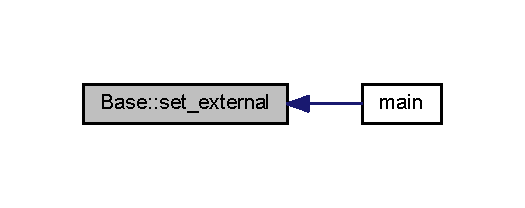
\includegraphics[width=252pt]{class_base_a87ec2d3dcffa1d22d4fe4f651f625d49_icgraph}
\end{center}
\end{figure}


The documentation for this class was generated from the following file\+:\begin{DoxyCompactItemize}
\item 
Doxy\+Test/\hyperlink{_classes_8h}{Classes.\+h}\end{DoxyCompactItemize}

\hypertarget{class_derived_one}{}\section{Derived\+One Class Reference}
\label{class_derived_one}\index{Derived\+One@{Derived\+One}}


{\ttfamily \#include $<$Classes.\+h$>$}



Inheritance diagram for Derived\+One\+:
\nopagebreak
\begin{figure}[H]
\begin{center}
\leavevmode
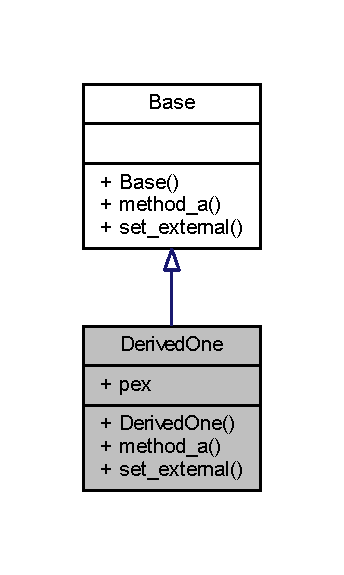
\includegraphics[width=165pt]{class_derived_one__inherit__graph}
\end{center}
\end{figure}


Collaboration diagram for Derived\+One\+:
\nopagebreak
\begin{figure}[H]
\begin{center}
\leavevmode
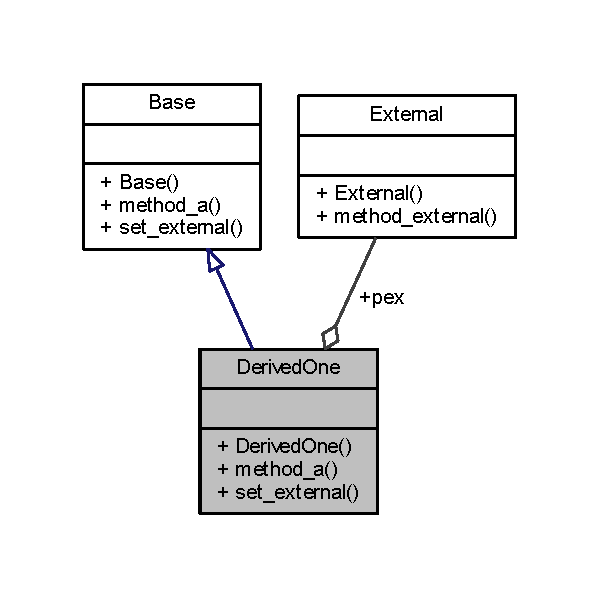
\includegraphics[width=288pt]{class_derived_one__coll__graph}
\end{center}
\end{figure}
\subsection*{Public Member Functions}
\begin{DoxyCompactItemize}
\item 
\hyperlink{class_derived_one_a10e249e537ac6388b0b1662a3dfea8f7}{Derived\+One} ()
\begin{DoxyCompactList}\small\item\em A constructor. \end{DoxyCompactList}\item 
virtual void \hyperlink{class_derived_one_a2843e6e6fd03fa84efda261cd1bbc10d}{method\+\_\+a} () const
\begin{DoxyCompactList}\small\item\em A normal member taking two arguments and returning an integer value. \end{DoxyCompactList}\item 
virtual void \hyperlink{class_derived_one_aa98db10f4b7ca15905aa82d942afe51b}{set\+\_\+external} (\hyperlink{class_external}{External} $\ast$ex)
\begin{DoxyCompactList}\small\item\em A normal member taking two arguments and returning an integer value. \end{DoxyCompactList}\end{DoxyCompactItemize}
\subsection*{Public Attributes}
\begin{DoxyCompactItemize}
\item 
\hyperlink{class_external}{External} $\ast$ \hyperlink{class_derived_one_aa55e1fcdabd28d0520ec6e68d530cc77}{pex}
\end{DoxyCompactItemize}


\subsection{Detailed Description}
\hyperlink{class_derived_one}{Derived\+One} class Level 2 class. \hyperlink{class_base}{Base} class description. 

Definition at line 86 of file Classes.\+h.



\subsection{Constructor \& Destructor Documentation}
\mbox{\Hypertarget{class_derived_one_a10e249e537ac6388b0b1662a3dfea8f7}\label{class_derived_one_a10e249e537ac6388b0b1662a3dfea8f7}} 
\index{Derived\+One@{Derived\+One}!Derived\+One@{Derived\+One}}
\index{Derived\+One@{Derived\+One}!Derived\+One@{Derived\+One}}
\subsubsection{\texorpdfstring{Derived\+One()}{DerivedOne()}}
{\footnotesize\ttfamily Derived\+One\+::\+Derived\+One (\begin{DoxyParamCaption}{ }\end{DoxyParamCaption})\hspace{0.3cm}{\ttfamily [inline]}}



A constructor. 

A more elaborate description of the constructor. 

Definition at line 93 of file Classes.\+h.



\subsection{Member Function Documentation}
\mbox{\Hypertarget{class_derived_one_a2843e6e6fd03fa84efda261cd1bbc10d}\label{class_derived_one_a2843e6e6fd03fa84efda261cd1bbc10d}} 
\index{Derived\+One@{Derived\+One}!method\+\_\+a@{method\+\_\+a}}
\index{method\+\_\+a@{method\+\_\+a}!Derived\+One@{Derived\+One}}
\subsubsection{\texorpdfstring{method\+\_\+a()}{method\_a()}}
{\footnotesize\ttfamily virtual void Derived\+One\+::method\+\_\+a (\begin{DoxyParamCaption}{ }\end{DoxyParamCaption}) const\hspace{0.3cm}{\ttfamily [inline]}, {\ttfamily [virtual]}}



A normal member taking two arguments and returning an integer value. 

nparam a an integer argument. nparam s a constant character pointer. nreturn The test results nsa Q\+Tstyle\+\_\+\+Test(), $\sim$\+Q\+Tstyle\+\_\+\+Test(), test\+Me\+Too() and public\+Var() 

Implements \hyperlink{class_base_ace5096ac7dfb41f2577321923e3048bf}{Base}.



Definition at line 102 of file Classes.\+h.

\mbox{\Hypertarget{class_derived_one_aa98db10f4b7ca15905aa82d942afe51b}\label{class_derived_one_aa98db10f4b7ca15905aa82d942afe51b}} 
\index{Derived\+One@{Derived\+One}!set\+\_\+external@{set\+\_\+external}}
\index{set\+\_\+external@{set\+\_\+external}!Derived\+One@{Derived\+One}}
\subsubsection{\texorpdfstring{set\+\_\+external()}{set\_external()}}
{\footnotesize\ttfamily virtual void Derived\+One\+::set\+\_\+external (\begin{DoxyParamCaption}\item[{\hyperlink{class_external}{External} $\ast$}]{ex }\end{DoxyParamCaption})\hspace{0.3cm}{\ttfamily [inline]}, {\ttfamily [virtual]}}



A normal member taking two arguments and returning an integer value. 

nparam a an integer argument. nparam s a constant character pointer. nreturn The test results nsa Q\+Tstyle\+\_\+\+Test(), $\sim$\+Q\+Tstyle\+\_\+\+Test(), test\+Me\+Too() and public\+Var() 

Implements \hyperlink{class_base_a87ec2d3dcffa1d22d4fe4f651f625d49}{Base}.



Definition at line 114 of file Classes.\+h.



\subsection{Member Data Documentation}
\mbox{\Hypertarget{class_derived_one_aa55e1fcdabd28d0520ec6e68d530cc77}\label{class_derived_one_aa55e1fcdabd28d0520ec6e68d530cc77}} 
\index{Derived\+One@{Derived\+One}!pex@{pex}}
\index{pex@{pex}!Derived\+One@{Derived\+One}}
\subsubsection{\texorpdfstring{pex}{pex}}
{\footnotesize\ttfamily \hyperlink{class_external}{External}$\ast$ Derived\+One\+::pex}



Definition at line 119 of file Classes.\+h.



The documentation for this class was generated from the following file\+:\begin{DoxyCompactItemize}
\item 
Doxy\+Test/\hyperlink{_classes_8h}{Classes.\+h}\end{DoxyCompactItemize}

\hypertarget{class_derived_three}{}\section{Derived\+Three Class Reference}
\label{class_derived_three}\index{Derived\+Three@{Derived\+Three}}


{\ttfamily \#include $<$Classes.\+h$>$}



Inheritance diagram for Derived\+Three\+:
\nopagebreak
\begin{figure}[H]
\begin{center}
\leavevmode
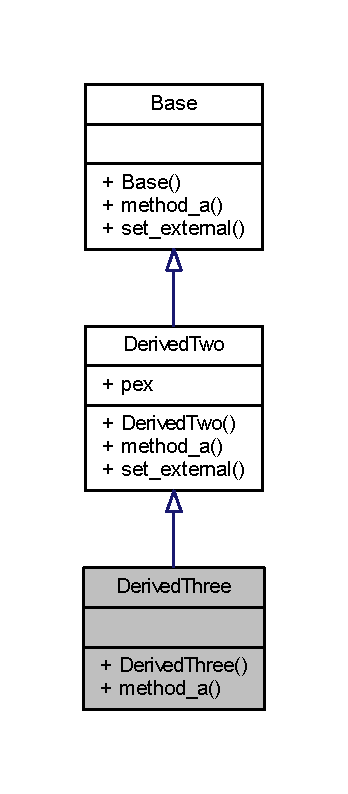
\includegraphics[width=167pt]{class_derived_three__inherit__graph}
\end{center}
\end{figure}


Collaboration diagram for Derived\+Three\+:
\nopagebreak
\begin{figure}[H]
\begin{center}
\leavevmode
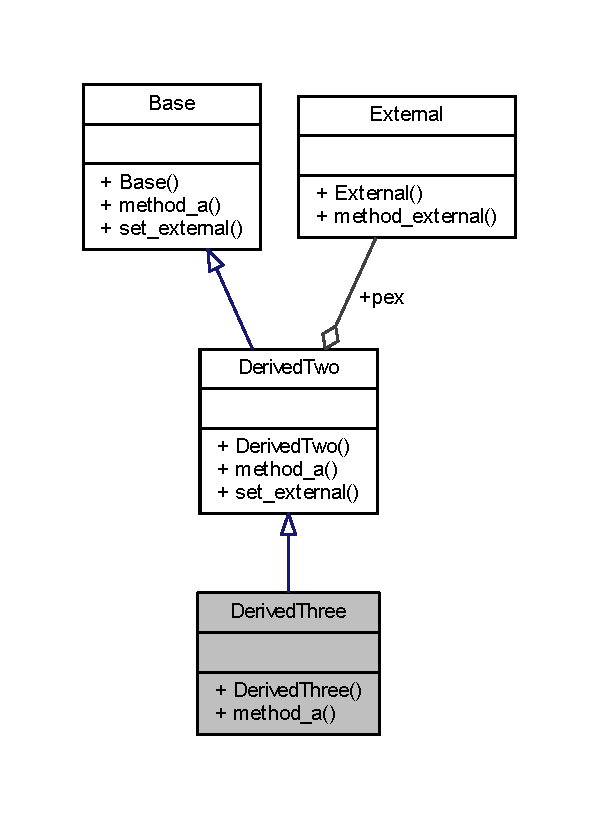
\includegraphics[width=288pt]{class_derived_three__coll__graph}
\end{center}
\end{figure}
\subsection*{Public Member Functions}
\begin{DoxyCompactItemize}
\item 
\hyperlink{class_derived_three_a7787b8ff6ade268d734edcdea3df5a2b}{Derived\+Three} ()
\begin{DoxyCompactList}\small\item\em A constructor. \end{DoxyCompactList}\item 
virtual void \hyperlink{class_derived_three_a74d2afff499ae551a424aa5d1da14620}{method\+\_\+a} () const
\begin{DoxyCompactList}\small\item\em A normal member taking two arguments and returning an integer value. \end{DoxyCompactList}\end{DoxyCompactItemize}
\subsection*{Additional Inherited Members}


\subsection{Detailed Description}
\hyperlink{class_derived_three}{Derived\+Three} class Level 3 class. \hyperlink{class_base}{Base} class description. 

Definition at line 168 of file Classes.\+h.



\subsection{Constructor \& Destructor Documentation}
\mbox{\Hypertarget{class_derived_three_a7787b8ff6ade268d734edcdea3df5a2b}\label{class_derived_three_a7787b8ff6ade268d734edcdea3df5a2b}} 
\index{Derived\+Three@{Derived\+Three}!Derived\+Three@{Derived\+Three}}
\index{Derived\+Three@{Derived\+Three}!Derived\+Three@{Derived\+Three}}
\subsubsection{\texorpdfstring{Derived\+Three()}{DerivedThree()}}
{\footnotesize\ttfamily Derived\+Three\+::\+Derived\+Three (\begin{DoxyParamCaption}{ }\end{DoxyParamCaption})\hspace{0.3cm}{\ttfamily [inline]}}



A constructor. 

A more elaborate description of the constructor. 

Definition at line 175 of file Classes.\+h.



\subsection{Member Function Documentation}
\mbox{\Hypertarget{class_derived_three_a74d2afff499ae551a424aa5d1da14620}\label{class_derived_three_a74d2afff499ae551a424aa5d1da14620}} 
\index{Derived\+Three@{Derived\+Three}!method\+\_\+a@{method\+\_\+a}}
\index{method\+\_\+a@{method\+\_\+a}!Derived\+Three@{Derived\+Three}}
\subsubsection{\texorpdfstring{method\+\_\+a()}{method\_a()}}
{\footnotesize\ttfamily virtual void Derived\+Three\+::method\+\_\+a (\begin{DoxyParamCaption}{ }\end{DoxyParamCaption}) const\hspace{0.3cm}{\ttfamily [inline]}, {\ttfamily [virtual]}}



A normal member taking two arguments and returning an integer value. 

nparam a an integer argument. nparam s a constant character pointer. nreturn The test results nsa Q\+Tstyle\+\_\+\+Test(), $\sim$\+Q\+Tstyle\+\_\+\+Test(), test\+Me\+Too() and public\+Var() 

Reimplemented from \hyperlink{class_derived_two_ae83bc07728d0af09413c6eb91c840e1d}{Derived\+Two}.



Definition at line 184 of file Classes.\+h.



The documentation for this class was generated from the following file\+:\begin{DoxyCompactItemize}
\item 
Doxy\+Test/\hyperlink{_classes_8h}{Classes.\+h}\end{DoxyCompactItemize}

\hypertarget{class_derived_two}{}\section{Derived\+Two Class Reference}
\label{class_derived_two}\index{Derived\+Two@{Derived\+Two}}


{\ttfamily \#include $<$Classes.\+h$>$}



Inheritance diagram for Derived\+Two\+:
\nopagebreak
\begin{figure}[H]
\begin{center}
\leavevmode
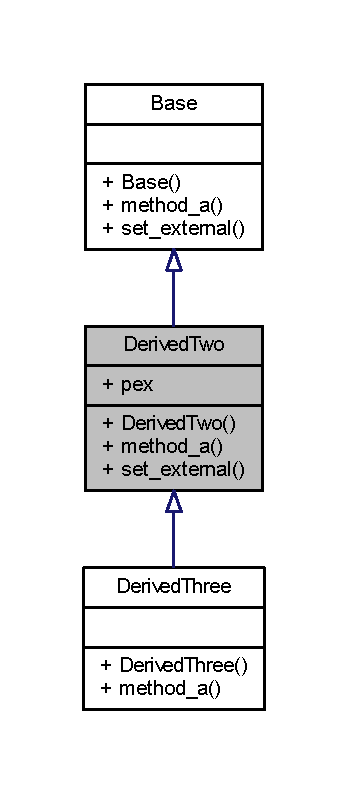
\includegraphics[width=167pt]{class_derived_two__inherit__graph}
\end{center}
\end{figure}


Collaboration diagram for Derived\+Two\+:
\nopagebreak
\begin{figure}[H]
\begin{center}
\leavevmode
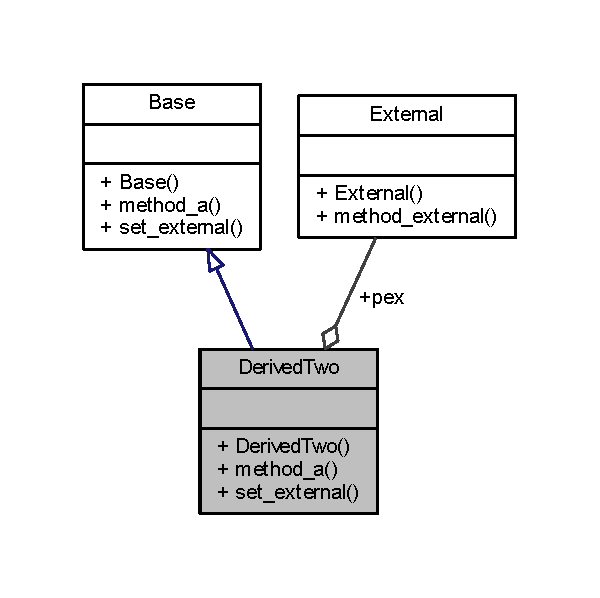
\includegraphics[width=288pt]{class_derived_two__coll__graph}
\end{center}
\end{figure}
\subsection*{Public Member Functions}
\begin{DoxyCompactItemize}
\item 
\hyperlink{class_derived_two_a9a3a078cc0cecad09409c8f812068b4c}{Derived\+Two} ()
\begin{DoxyCompactList}\small\item\em A constructor. \end{DoxyCompactList}\item 
virtual void \hyperlink{class_derived_two_ae83bc07728d0af09413c6eb91c840e1d}{method\+\_\+a} () const
\begin{DoxyCompactList}\small\item\em A normal member taking two arguments and returning an integer value. \end{DoxyCompactList}\item 
virtual void \hyperlink{class_derived_two_a84a5387e229abb415d74fb4ed8a5d913}{set\+\_\+external} (\hyperlink{class_external}{External} $\ast$ex)
\begin{DoxyCompactList}\small\item\em A normal member taking two arguments and returning an integer value. \end{DoxyCompactList}\end{DoxyCompactItemize}
\subsection*{Public Attributes}
\begin{DoxyCompactItemize}
\item 
\hyperlink{class_external}{External} $\ast$ \hyperlink{class_derived_two_a802d77367aae0f23c503def0befd6a88}{pex}
\end{DoxyCompactItemize}


\subsection{Detailed Description}
\hyperlink{class_derived_two}{Derived\+Two} class Level 2 class. \hyperlink{class_base}{Base} class description. 

Definition at line 127 of file Classes.\+h.



\subsection{Constructor \& Destructor Documentation}
\mbox{\Hypertarget{class_derived_two_a9a3a078cc0cecad09409c8f812068b4c}\label{class_derived_two_a9a3a078cc0cecad09409c8f812068b4c}} 
\index{Derived\+Two@{Derived\+Two}!Derived\+Two@{Derived\+Two}}
\index{Derived\+Two@{Derived\+Two}!Derived\+Two@{Derived\+Two}}
\subsubsection{\texorpdfstring{Derived\+Two()}{DerivedTwo()}}
{\footnotesize\ttfamily Derived\+Two\+::\+Derived\+Two (\begin{DoxyParamCaption}{ }\end{DoxyParamCaption})\hspace{0.3cm}{\ttfamily [inline]}}



A constructor. 

A more elaborate description of the constructor. 

Definition at line 134 of file Classes.\+h.



\subsection{Member Function Documentation}
\mbox{\Hypertarget{class_derived_two_ae83bc07728d0af09413c6eb91c840e1d}\label{class_derived_two_ae83bc07728d0af09413c6eb91c840e1d}} 
\index{Derived\+Two@{Derived\+Two}!method\+\_\+a@{method\+\_\+a}}
\index{method\+\_\+a@{method\+\_\+a}!Derived\+Two@{Derived\+Two}}
\subsubsection{\texorpdfstring{method\+\_\+a()}{method\_a()}}
{\footnotesize\ttfamily virtual void Derived\+Two\+::method\+\_\+a (\begin{DoxyParamCaption}{ }\end{DoxyParamCaption}) const\hspace{0.3cm}{\ttfamily [inline]}, {\ttfamily [virtual]}}



A normal member taking two arguments and returning an integer value. 

nparam a an integer argument. nparam s a constant character pointer. nreturn The test results nsa Q\+Tstyle\+\_\+\+Test(), $\sim$\+Q\+Tstyle\+\_\+\+Test(), test\+Me\+Too() and public\+Var() 

Implements \hyperlink{class_base_ace5096ac7dfb41f2577321923e3048bf}{Base}.



Reimplemented in \hyperlink{class_derived_three_a74d2afff499ae551a424aa5d1da14620}{Derived\+Three}.



Definition at line 143 of file Classes.\+h.

\mbox{\Hypertarget{class_derived_two_a84a5387e229abb415d74fb4ed8a5d913}\label{class_derived_two_a84a5387e229abb415d74fb4ed8a5d913}} 
\index{Derived\+Two@{Derived\+Two}!set\+\_\+external@{set\+\_\+external}}
\index{set\+\_\+external@{set\+\_\+external}!Derived\+Two@{Derived\+Two}}
\subsubsection{\texorpdfstring{set\+\_\+external()}{set\_external()}}
{\footnotesize\ttfamily virtual void Derived\+Two\+::set\+\_\+external (\begin{DoxyParamCaption}\item[{\hyperlink{class_external}{External} $\ast$}]{ex }\end{DoxyParamCaption})\hspace{0.3cm}{\ttfamily [inline]}, {\ttfamily [virtual]}}



A normal member taking two arguments and returning an integer value. 

nparam a an integer argument. nparam s a constant character pointer. nreturn The test results nsa Q\+Tstyle\+\_\+\+Test(), $\sim$\+Q\+Tstyle\+\_\+\+Test(), test\+Me\+Too() and public\+Var() 

Implements \hyperlink{class_base_a87ec2d3dcffa1d22d4fe4f651f625d49}{Base}.



Definition at line 155 of file Classes.\+h.



\subsection{Member Data Documentation}
\mbox{\Hypertarget{class_derived_two_a802d77367aae0f23c503def0befd6a88}\label{class_derived_two_a802d77367aae0f23c503def0befd6a88}} 
\index{Derived\+Two@{Derived\+Two}!pex@{pex}}
\index{pex@{pex}!Derived\+Two@{Derived\+Two}}
\subsubsection{\texorpdfstring{pex}{pex}}
{\footnotesize\ttfamily \hyperlink{class_external}{External}$\ast$ Derived\+Two\+::pex}



Definition at line 160 of file Classes.\+h.



The documentation for this class was generated from the following file\+:\begin{DoxyCompactItemize}
\item 
Doxy\+Test/\hyperlink{_classes_8h}{Classes.\+h}\end{DoxyCompactItemize}

\hypertarget{class_external}{}\section{External Class Reference}
\label{class_external}\index{External@{External}}


{\ttfamily \#include $<$Classes.\+h$>$}



Inheritance diagram for External\+:
\nopagebreak
\begin{figure}[H]
\begin{center}
\leavevmode
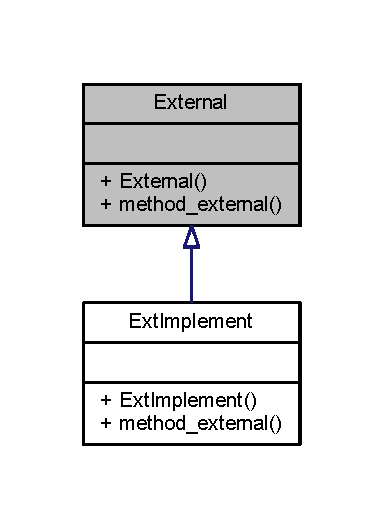
\includegraphics[width=184pt]{class_external__inherit__graph}
\end{center}
\end{figure}


Collaboration diagram for External\+:
\nopagebreak
\begin{figure}[H]
\begin{center}
\leavevmode
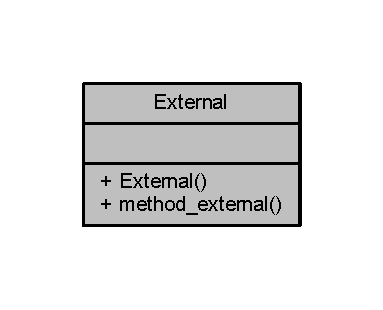
\includegraphics[width=184pt]{class_external__coll__graph}
\end{center}
\end{figure}
\subsection*{Public Member Functions}
\begin{DoxyCompactItemize}
\item 
\hyperlink{class_external_ad2872b94971bb19971df29b1c04036fc}{External} ()
\begin{DoxyCompactList}\small\item\em A constructor. \end{DoxyCompactList}\item 
virtual void \hyperlink{class_external_a6bda85aa1f6f1396469261bd13d39e72}{method\+\_\+external} () const =0
\begin{DoxyCompactList}\small\item\em A normal member taking two arguments and returning an integer value. \end{DoxyCompactList}\end{DoxyCompactItemize}


\subsection{Detailed Description}
\hyperlink{class_external}{External} class Some external class. \hyperlink{class_base}{Base} class description. 

Definition at line 9 of file Classes.\+h.



\subsection{Constructor \& Destructor Documentation}
\mbox{\Hypertarget{class_external_ad2872b94971bb19971df29b1c04036fc}\label{class_external_ad2872b94971bb19971df29b1c04036fc}} 
\index{External@{External}!External@{External}}
\index{External@{External}!External@{External}}
\subsubsection{\texorpdfstring{External()}{External()}}
{\footnotesize\ttfamily External\+::\+External (\begin{DoxyParamCaption}{ }\end{DoxyParamCaption})\hspace{0.3cm}{\ttfamily [inline]}}



A constructor. 

A more elaborate description of the constructor. 

Definition at line 16 of file Classes.\+h.

Here is the call graph for this function\+:
\nopagebreak
\begin{figure}[H]
\begin{center}
\leavevmode
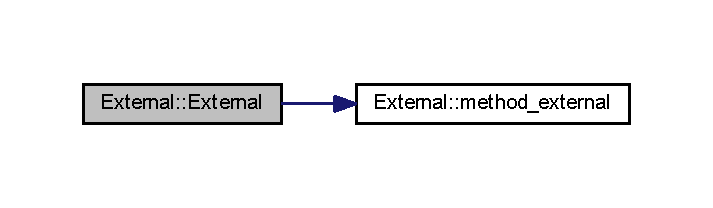
\includegraphics[width=342pt]{class_external_ad2872b94971bb19971df29b1c04036fc_cgraph}
\end{center}
\end{figure}


\subsection{Member Function Documentation}
\mbox{\Hypertarget{class_external_a6bda85aa1f6f1396469261bd13d39e72}\label{class_external_a6bda85aa1f6f1396469261bd13d39e72}} 
\index{External@{External}!method\+\_\+external@{method\+\_\+external}}
\index{method\+\_\+external@{method\+\_\+external}!External@{External}}
\subsubsection{\texorpdfstring{method\+\_\+external()}{method\_external()}}
{\footnotesize\ttfamily virtual void External\+::method\+\_\+external (\begin{DoxyParamCaption}{ }\end{DoxyParamCaption}) const\hspace{0.3cm}{\ttfamily [pure virtual]}}



A normal member taking two arguments and returning an integer value. 

nparam a an integer argument. nparam s a constant character pointer. nreturn The test results nsa Q\+Tstyle\+\_\+\+Test(), $\sim$\+Q\+Tstyle\+\_\+\+Test(), test\+Me\+Too() and public\+Var() 

Implemented in \hyperlink{class_ext_implement_a5f41afb83e49e92542b031aecfd097a9}{Ext\+Implement}.

Here is the caller graph for this function\+:
\nopagebreak
\begin{figure}[H]
\begin{center}
\leavevmode
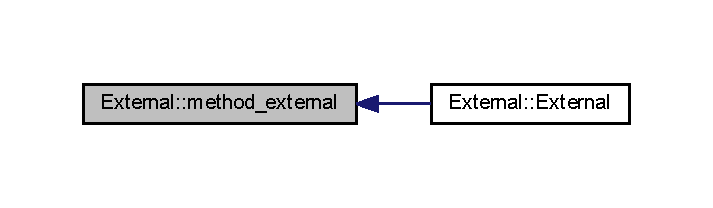
\includegraphics[width=342pt]{class_external_a6bda85aa1f6f1396469261bd13d39e72_icgraph}
\end{center}
\end{figure}


The documentation for this class was generated from the following file\+:\begin{DoxyCompactItemize}
\item 
Doxy\+Test/\hyperlink{_classes_8h}{Classes.\+h}\end{DoxyCompactItemize}

\hypertarget{class_ext_implement}{}\section{Ext\+Implement Class Reference}
\label{class_ext_implement}\index{Ext\+Implement@{Ext\+Implement}}


{\ttfamily \#include $<$Classes.\+h$>$}



Inheritance diagram for Ext\+Implement\+:
\nopagebreak
\begin{figure}[H]
\begin{center}
\leavevmode
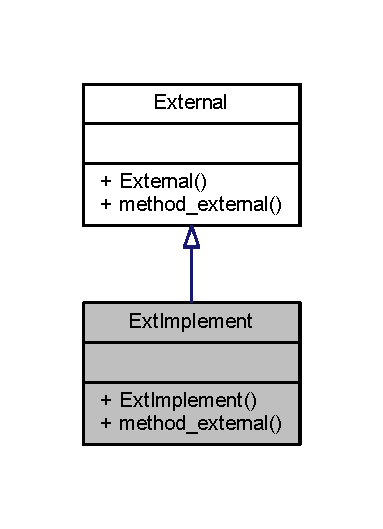
\includegraphics[width=184pt]{class_ext_implement__inherit__graph}
\end{center}
\end{figure}


Collaboration diagram for Ext\+Implement\+:
\nopagebreak
\begin{figure}[H]
\begin{center}
\leavevmode
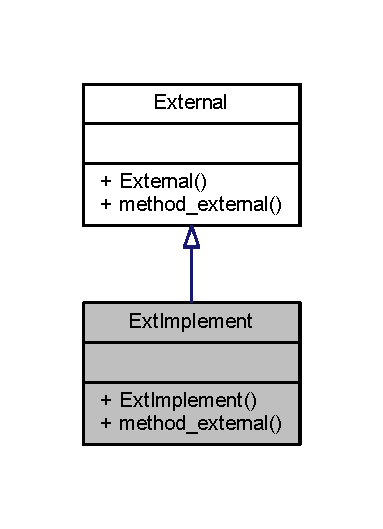
\includegraphics[width=184pt]{class_ext_implement__coll__graph}
\end{center}
\end{figure}
\subsection*{Public Member Functions}
\begin{DoxyCompactItemize}
\item 
\hyperlink{class_ext_implement_a298c71d0ba5e16fd571dffeaccde6902}{Ext\+Implement} ()
\begin{DoxyCompactList}\small\item\em A constructor. \end{DoxyCompactList}\item 
virtual void \hyperlink{class_ext_implement_a5f41afb83e49e92542b031aecfd097a9}{method\+\_\+external} () const
\begin{DoxyCompactList}\small\item\em A normal member taking two arguments and returning an integer value. \end{DoxyCompactList}\end{DoxyCompactItemize}


\subsection{Detailed Description}
\hyperlink{class_ext_implement}{Ext\+Implement} class Some external class. \hyperlink{class_base}{Base} class description. 

Definition at line 32 of file Classes.\+h.



\subsection{Constructor \& Destructor Documentation}
\mbox{\Hypertarget{class_ext_implement_a298c71d0ba5e16fd571dffeaccde6902}\label{class_ext_implement_a298c71d0ba5e16fd571dffeaccde6902}} 
\index{Ext\+Implement@{Ext\+Implement}!Ext\+Implement@{Ext\+Implement}}
\index{Ext\+Implement@{Ext\+Implement}!Ext\+Implement@{Ext\+Implement}}
\subsubsection{\texorpdfstring{Ext\+Implement()}{ExtImplement()}}
{\footnotesize\ttfamily Ext\+Implement\+::\+Ext\+Implement (\begin{DoxyParamCaption}{ }\end{DoxyParamCaption})\hspace{0.3cm}{\ttfamily [inline]}}



A constructor. 

A more elaborate description of the constructor. 

Definition at line 39 of file Classes.\+h.



\subsection{Member Function Documentation}
\mbox{\Hypertarget{class_ext_implement_a5f41afb83e49e92542b031aecfd097a9}\label{class_ext_implement_a5f41afb83e49e92542b031aecfd097a9}} 
\index{Ext\+Implement@{Ext\+Implement}!method\+\_\+external@{method\+\_\+external}}
\index{method\+\_\+external@{method\+\_\+external}!Ext\+Implement@{Ext\+Implement}}
\subsubsection{\texorpdfstring{method\+\_\+external()}{method\_external()}}
{\footnotesize\ttfamily virtual void Ext\+Implement\+::method\+\_\+external (\begin{DoxyParamCaption}{ }\end{DoxyParamCaption}) const\hspace{0.3cm}{\ttfamily [inline]}, {\ttfamily [virtual]}}



A normal member taking two arguments and returning an integer value. 

nparam a an integer argument. nparam s a constant character pointer. nreturn The test results nsa Q\+Tstyle\+\_\+\+Test(), $\sim$\+Q\+Tstyle\+\_\+\+Test(), test\+Me\+Too() and public\+Var() 

Implements \hyperlink{class_external_a6bda85aa1f6f1396469261bd13d39e72}{External}.



Definition at line 48 of file Classes.\+h.



The documentation for this class was generated from the following file\+:\begin{DoxyCompactItemize}
\item 
Doxy\+Test/\hyperlink{_classes_8h}{Classes.\+h}\end{DoxyCompactItemize}

\chapter{File Documentation}
\hypertarget{_classes_8cpp}{}\section{Doxy\+Test/\+Classes.cpp File Reference}
\label{_classes_8cpp}\index{Doxy\+Test/\+Classes.\+cpp@{Doxy\+Test/\+Classes.\+cpp}}
{\ttfamily \#include \char`\"{}stdafx.\+h\char`\"{}}\newline
{\ttfamily \#include \char`\"{}Classes.\+h\char`\"{}}\newline
Include dependency graph for Classes.\+cpp\+:
\nopagebreak
\begin{figure}[H]
\begin{center}
\leavevmode
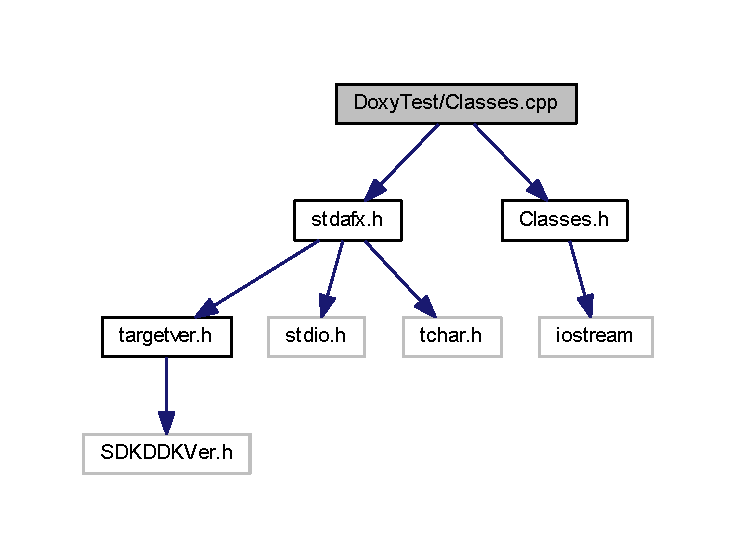
\includegraphics[width=350pt]{_classes_8cpp__incl}
\end{center}
\end{figure}

\hypertarget{_classes_8h}{}\section{Doxy\+Test/\+Classes.h File Reference}
\label{_classes_8h}\index{Doxy\+Test/\+Classes.\+h@{Doxy\+Test/\+Classes.\+h}}
{\ttfamily \#include $<$iostream$>$}\newline
Include dependency graph for Classes.\+h\+:
\nopagebreak
\begin{figure}[H]
\begin{center}
\leavevmode
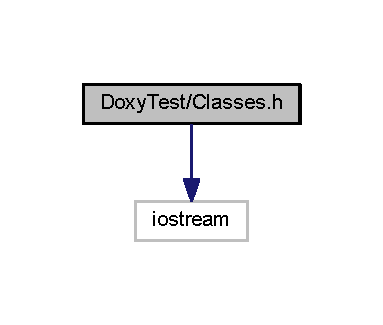
\includegraphics[width=184pt]{_classes_8h__incl}
\end{center}
\end{figure}
This graph shows which files directly or indirectly include this file\+:
\nopagebreak
\begin{figure}[H]
\begin{center}
\leavevmode
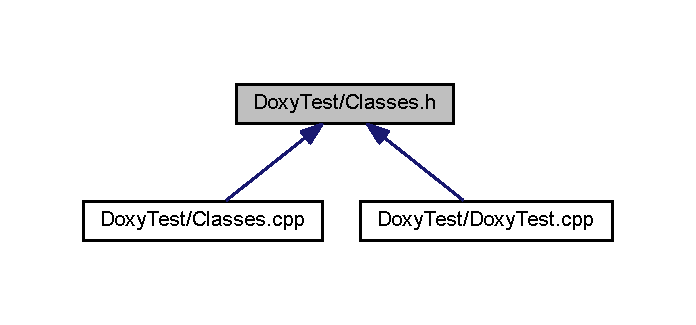
\includegraphics[width=334pt]{_classes_8h__dep__incl}
\end{center}
\end{figure}
\subsection*{Classes}
\begin{DoxyCompactItemize}
\item 
class \hyperlink{class_external}{External}
\item 
class \hyperlink{class_ext_implement}{Ext\+Implement}
\item 
class \hyperlink{class_base}{Base}
\item 
class \hyperlink{class_derived_one}{Derived\+One}
\item 
class \hyperlink{class_derived_two}{Derived\+Two}
\item 
class \hyperlink{class_derived_three}{Derived\+Three}
\end{DoxyCompactItemize}

\hypertarget{_doxy_test_8cpp}{}\section{Doxy\+Test/\+Doxy\+Test.cpp File Reference}
\label{_doxy_test_8cpp}\index{Doxy\+Test/\+Doxy\+Test.\+cpp@{Doxy\+Test/\+Doxy\+Test.\+cpp}}
{\ttfamily \#include \char`\"{}stdafx.\+h\char`\"{}}\newline
{\ttfamily \#include \char`\"{}Classes.\+h\char`\"{}}\newline
Include dependency graph for Doxy\+Test.\+cpp\+:
\nopagebreak
\begin{figure}[H]
\begin{center}
\leavevmode
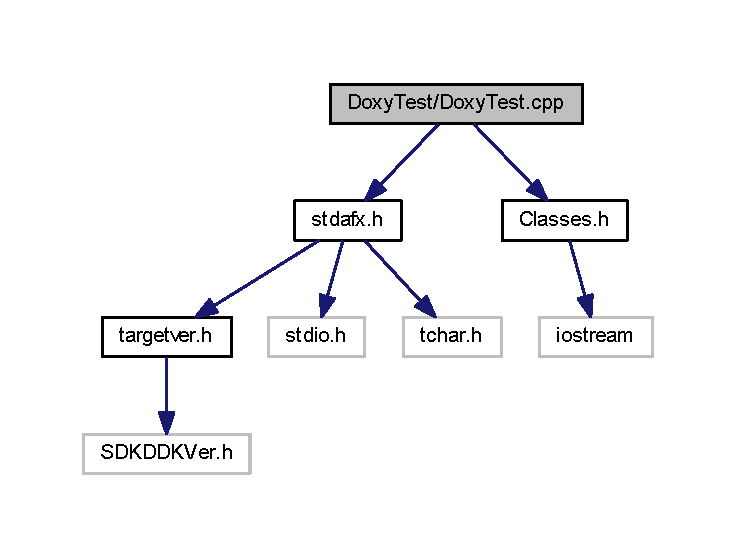
\includegraphics[width=350pt]{_doxy_test_8cpp__incl}
\end{center}
\end{figure}
\subsection*{Functions}
\begin{DoxyCompactItemize}
\item 
int \hyperlink{_doxy_test_8cpp_ae66f6b31b5ad750f1fe042a706a4e3d4}{main} ()
\end{DoxyCompactItemize}


\subsection{Function Documentation}
\mbox{\Hypertarget{_doxy_test_8cpp_ae66f6b31b5ad750f1fe042a706a4e3d4}\label{_doxy_test_8cpp_ae66f6b31b5ad750f1fe042a706a4e3d4}} 
\index{Doxy\+Test.\+cpp@{Doxy\+Test.\+cpp}!main@{main}}
\index{main@{main}!Doxy\+Test.\+cpp@{Doxy\+Test.\+cpp}}
\subsubsection{\texorpdfstring{main()}{main()}}
{\footnotesize\ttfamily int main (\begin{DoxyParamCaption}{ }\end{DoxyParamCaption})}



Definition at line 7 of file Doxy\+Test.\+cpp.

Here is the call graph for this function\+:
\nopagebreak
\begin{figure}[H]
\begin{center}
\leavevmode
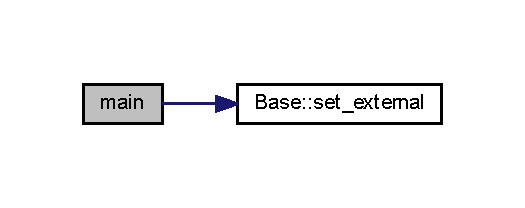
\includegraphics[width=252pt]{_doxy_test_8cpp_ae66f6b31b5ad750f1fe042a706a4e3d4_cgraph}
\end{center}
\end{figure}

\hypertarget{stdafx_8cpp}{}\section{Doxy\+Test/stdafx.cpp File Reference}
\label{stdafx_8cpp}\index{Doxy\+Test/stdafx.\+cpp@{Doxy\+Test/stdafx.\+cpp}}
{\ttfamily \#include \char`\"{}stdafx.\+h\char`\"{}}\newline
Include dependency graph for stdafx.\+cpp\+:
\nopagebreak
\begin{figure}[H]
\begin{center}
\leavevmode
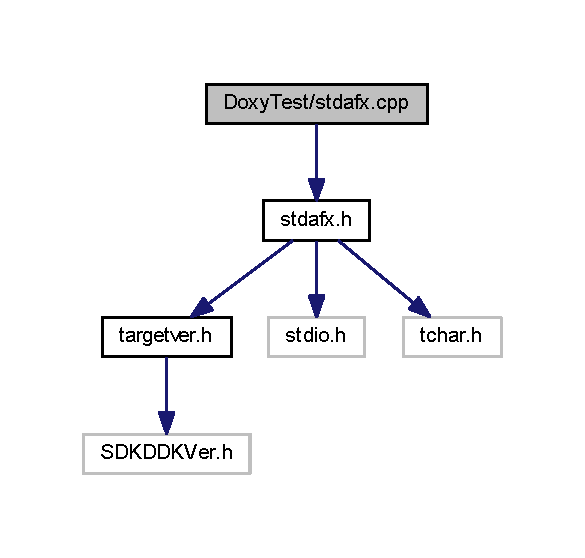
\includegraphics[width=281pt]{stdafx_8cpp__incl}
\end{center}
\end{figure}

\hypertarget{stdafx_8h}{}\section{Doxy\+Test/stdafx.h File Reference}
\label{stdafx_8h}\index{Doxy\+Test/stdafx.\+h@{Doxy\+Test/stdafx.\+h}}
{\ttfamily \#include \char`\"{}targetver.\+h\char`\"{}}\newline
{\ttfamily \#include $<$stdio.\+h$>$}\newline
{\ttfamily \#include $<$tchar.\+h$>$}\newline
Include dependency graph for stdafx.\+h\+:
\nopagebreak
\begin{figure}[H]
\begin{center}
\leavevmode
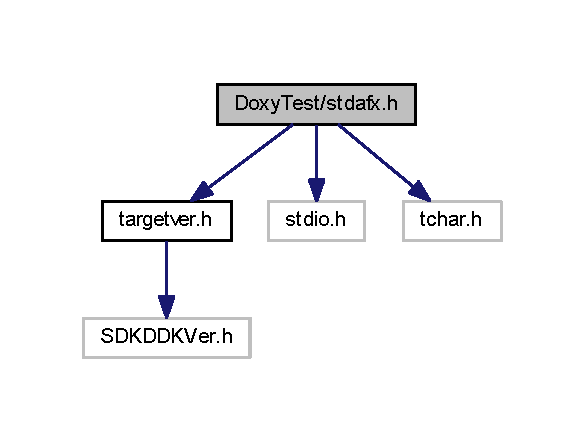
\includegraphics[width=281pt]{stdafx_8h__incl}
\end{center}
\end{figure}
This graph shows which files directly or indirectly include this file\+:
\nopagebreak
\begin{figure}[H]
\begin{center}
\leavevmode
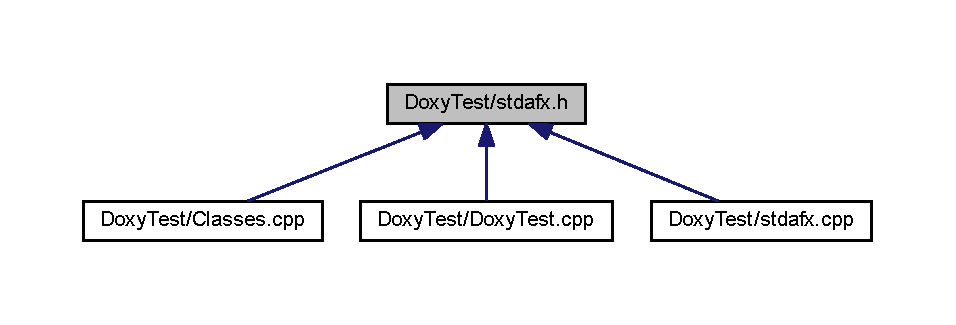
\includegraphics[width=350pt]{stdafx_8h__dep__incl}
\end{center}
\end{figure}

\hypertarget{targetver_8h}{}\section{Doxy\+Test/targetver.h File Reference}
\label{targetver_8h}\index{Doxy\+Test/targetver.\+h@{Doxy\+Test/targetver.\+h}}
{\ttfamily \#include $<$S\+D\+K\+D\+D\+K\+Ver.\+h$>$}\newline
Include dependency graph for targetver.\+h\+:
\nopagebreak
\begin{figure}[H]
\begin{center}
\leavevmode
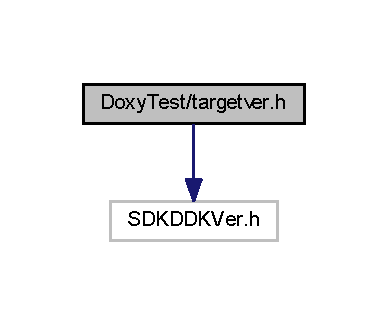
\includegraphics[width=186pt]{targetver_8h__incl}
\end{center}
\end{figure}
This graph shows which files directly or indirectly include this file\+:
\nopagebreak
\begin{figure}[H]
\begin{center}
\leavevmode
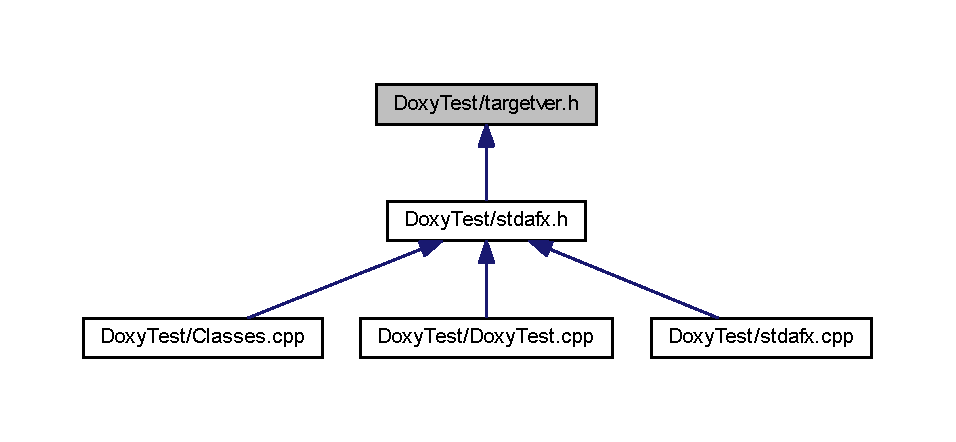
\includegraphics[width=350pt]{targetver_8h__dep__incl}
\end{center}
\end{figure}

%--- End generated contents ---

% Index
\backmatter
\newpage
\phantomsection
\clearemptydoublepage
\addcontentsline{toc}{chapter}{Index}
\printindex

\end{document}
